\Exhibit{MediumDistributedExplained}{%
    Screenshots of popular blogs explaining that the `Distributed' label
    is the sign of curation on Medium%
}

Medium Help Center did not tell how to recognize a curated article on the statistics pages.
Instead, these popular blogs can be used.
Multiple independent sources are given for assurance.

`Better Marketing' is a publication on Medium with 119 thousand followers:

\begin{center}
    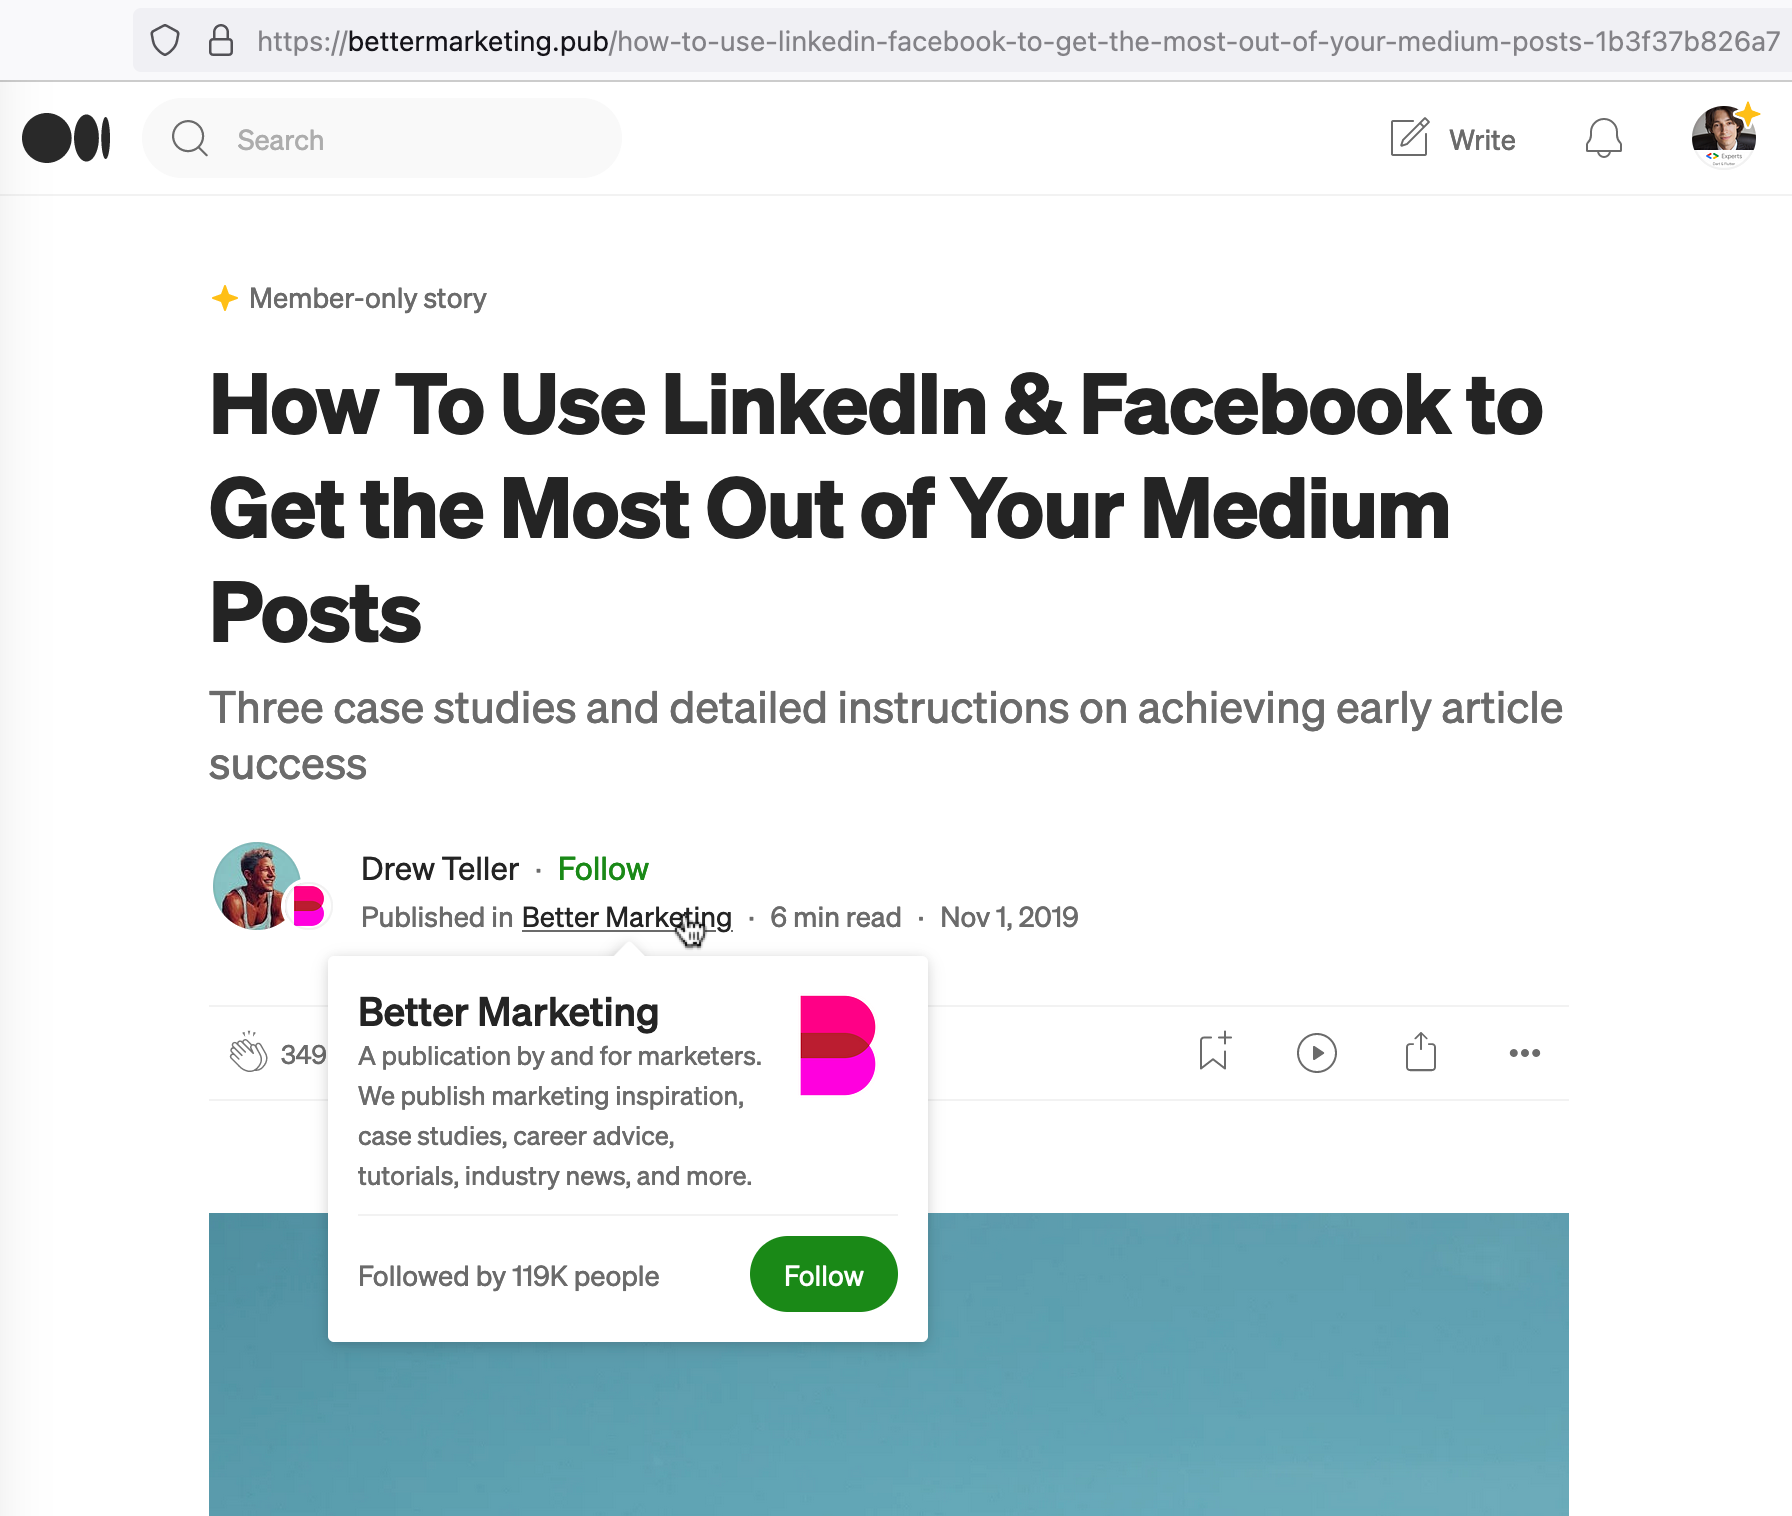
\includegraphics[width=\textwidth]{bettermarketing-top}
\end{center}

It published this article that explains this in its middle part:

\begin{center}
    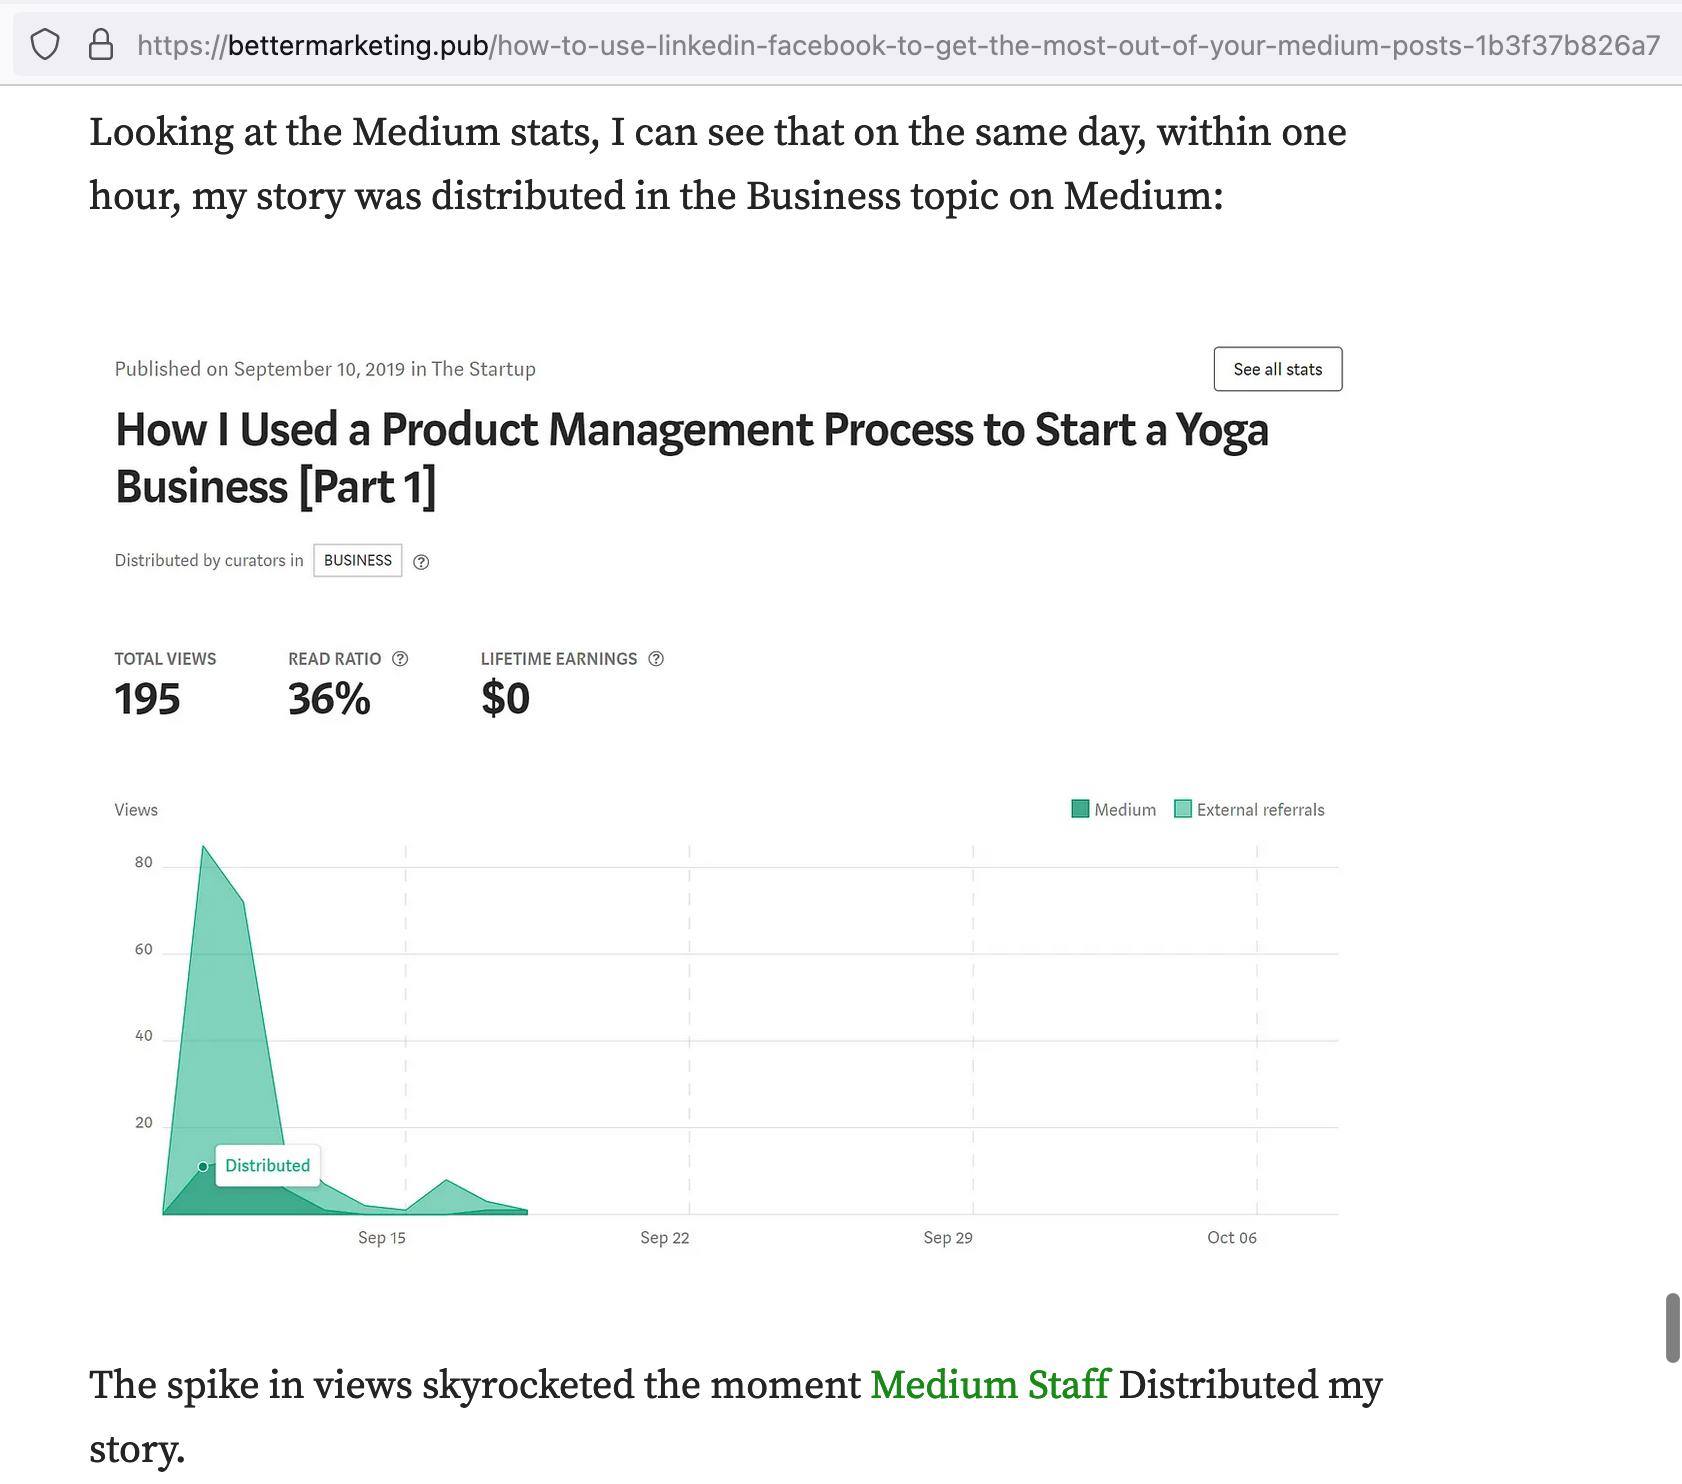
\includegraphics[width=\textwidth]{bettermarketing-content}
\end{center}
\pagebreak


This post in TheSideBlogger.com confirms that and explicitly highlights the signs.
It also confirms that the program was shut down in mid-2022.

\begin{center}
    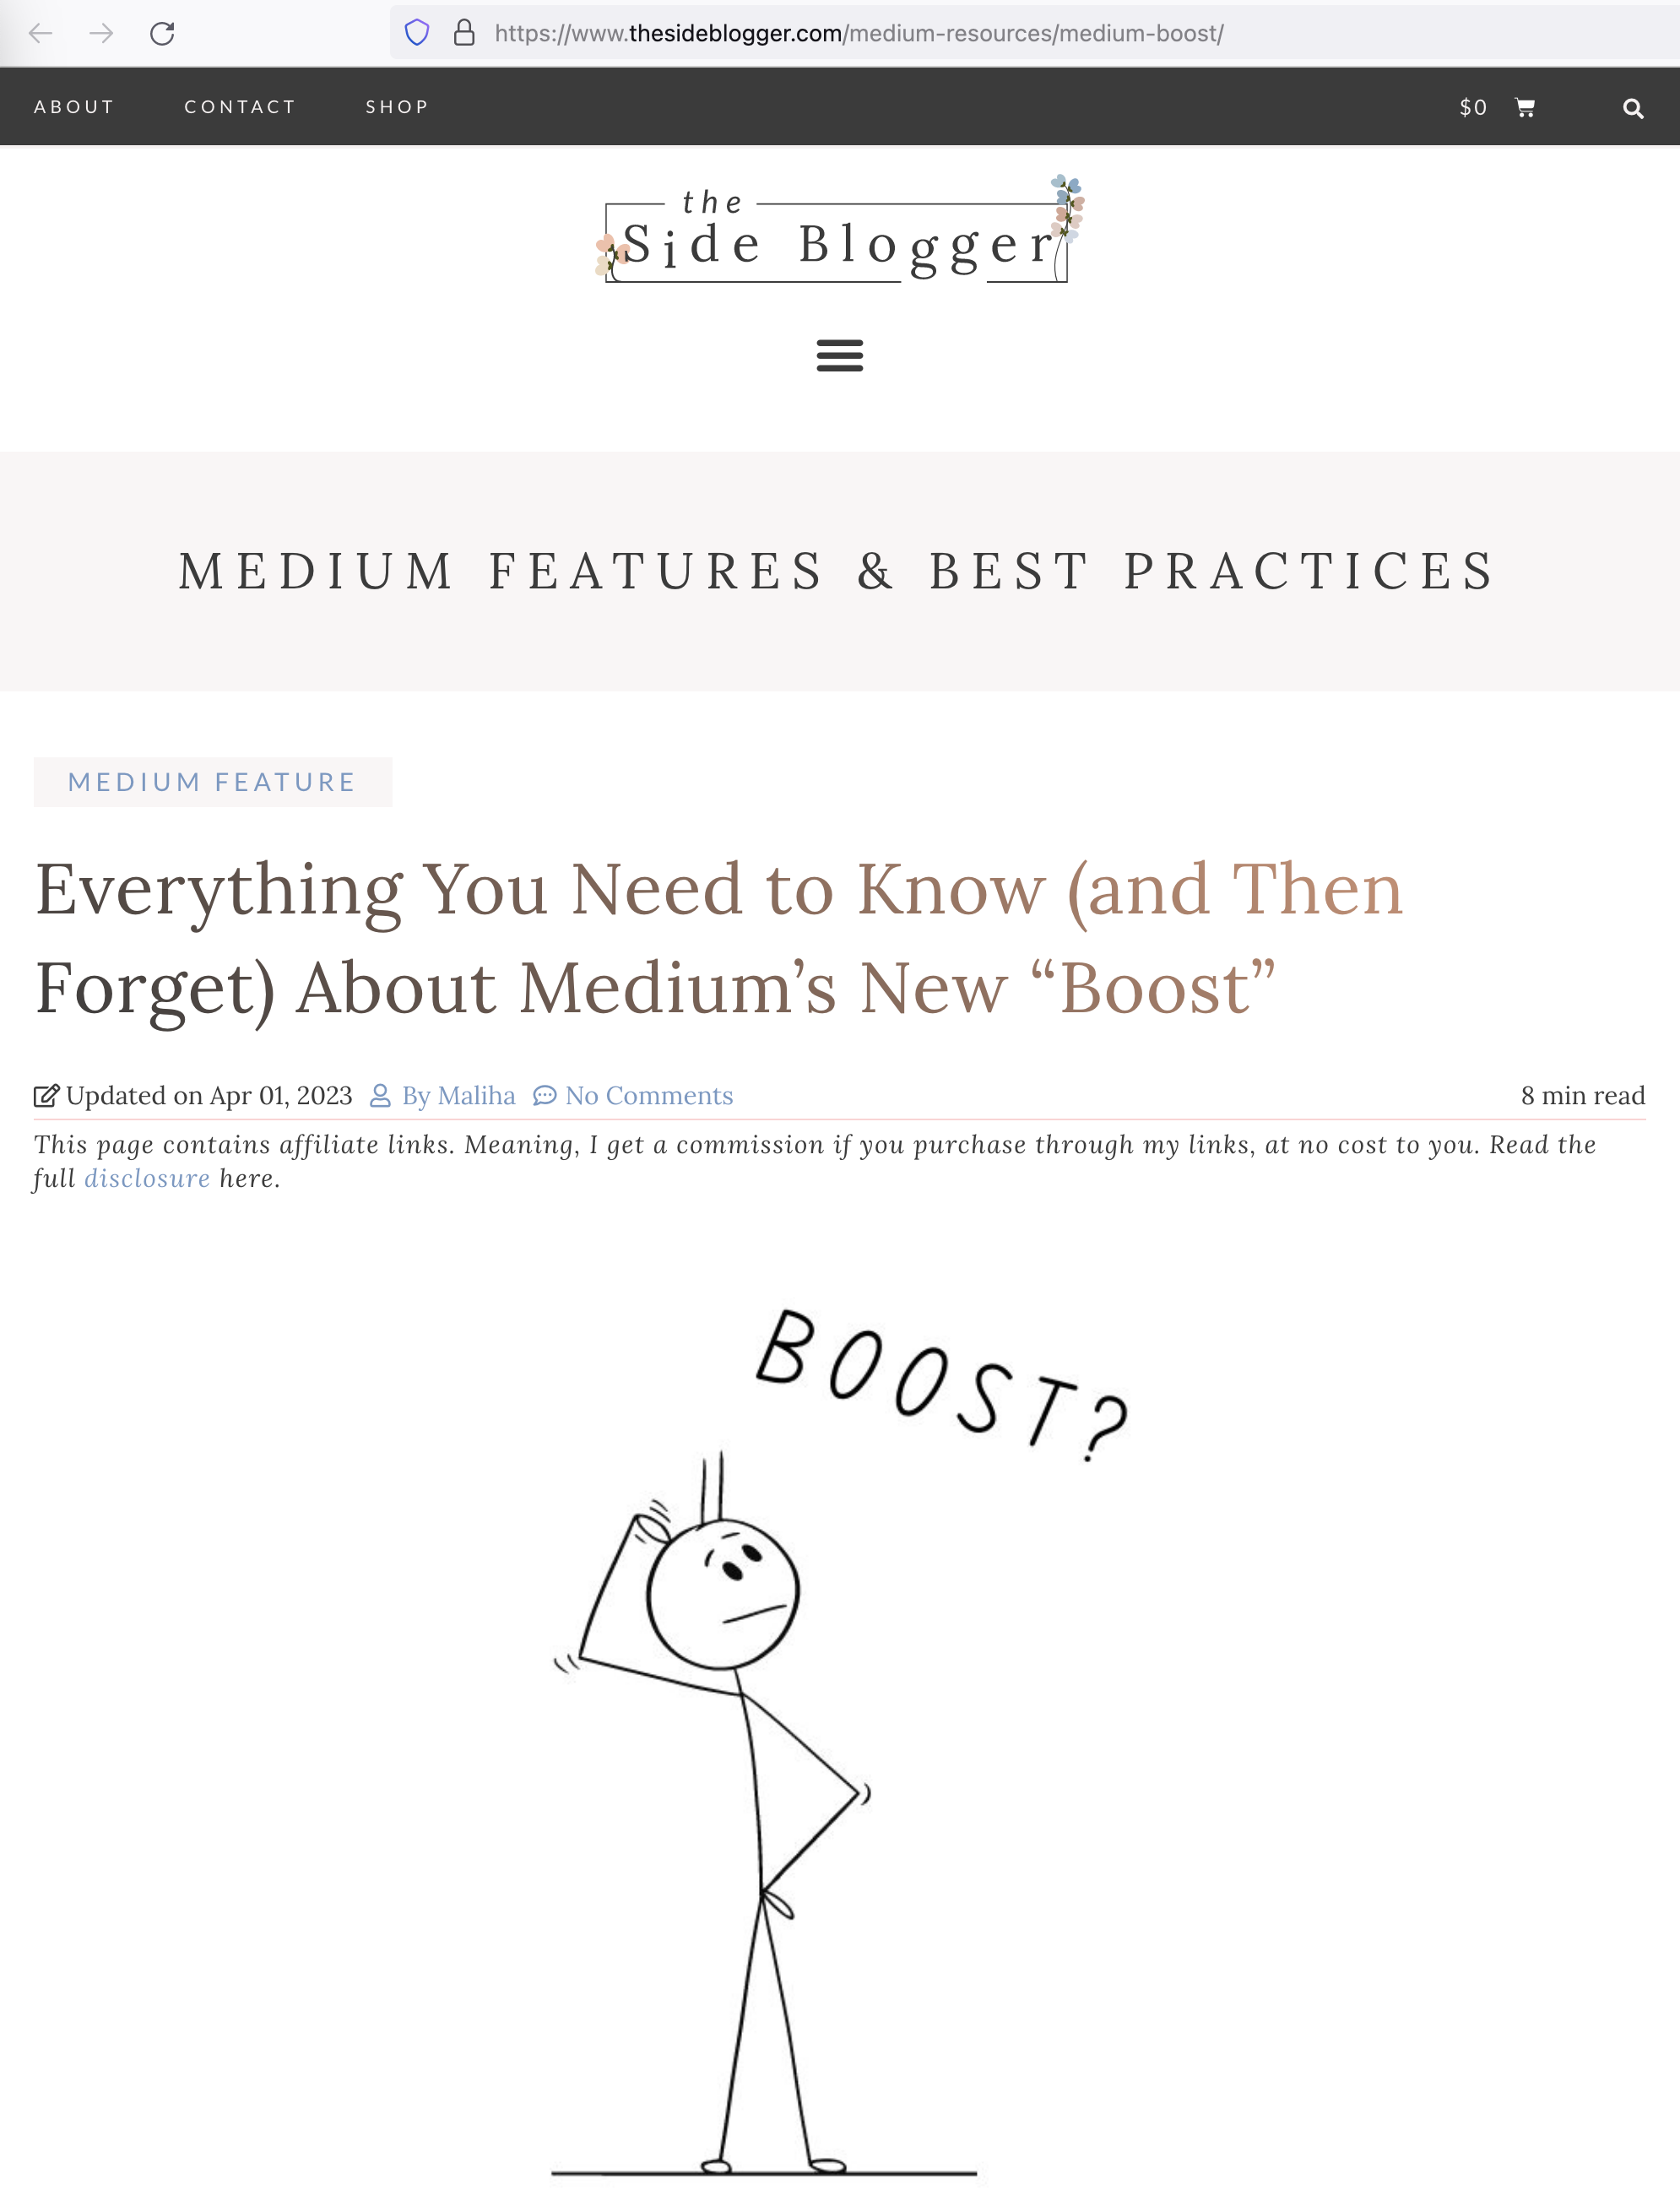
\includegraphics[width=38em]{thesideblogger-p1}
\end{center}
\WillContinue
\pagebreak

\Continuing
\begin{center}
    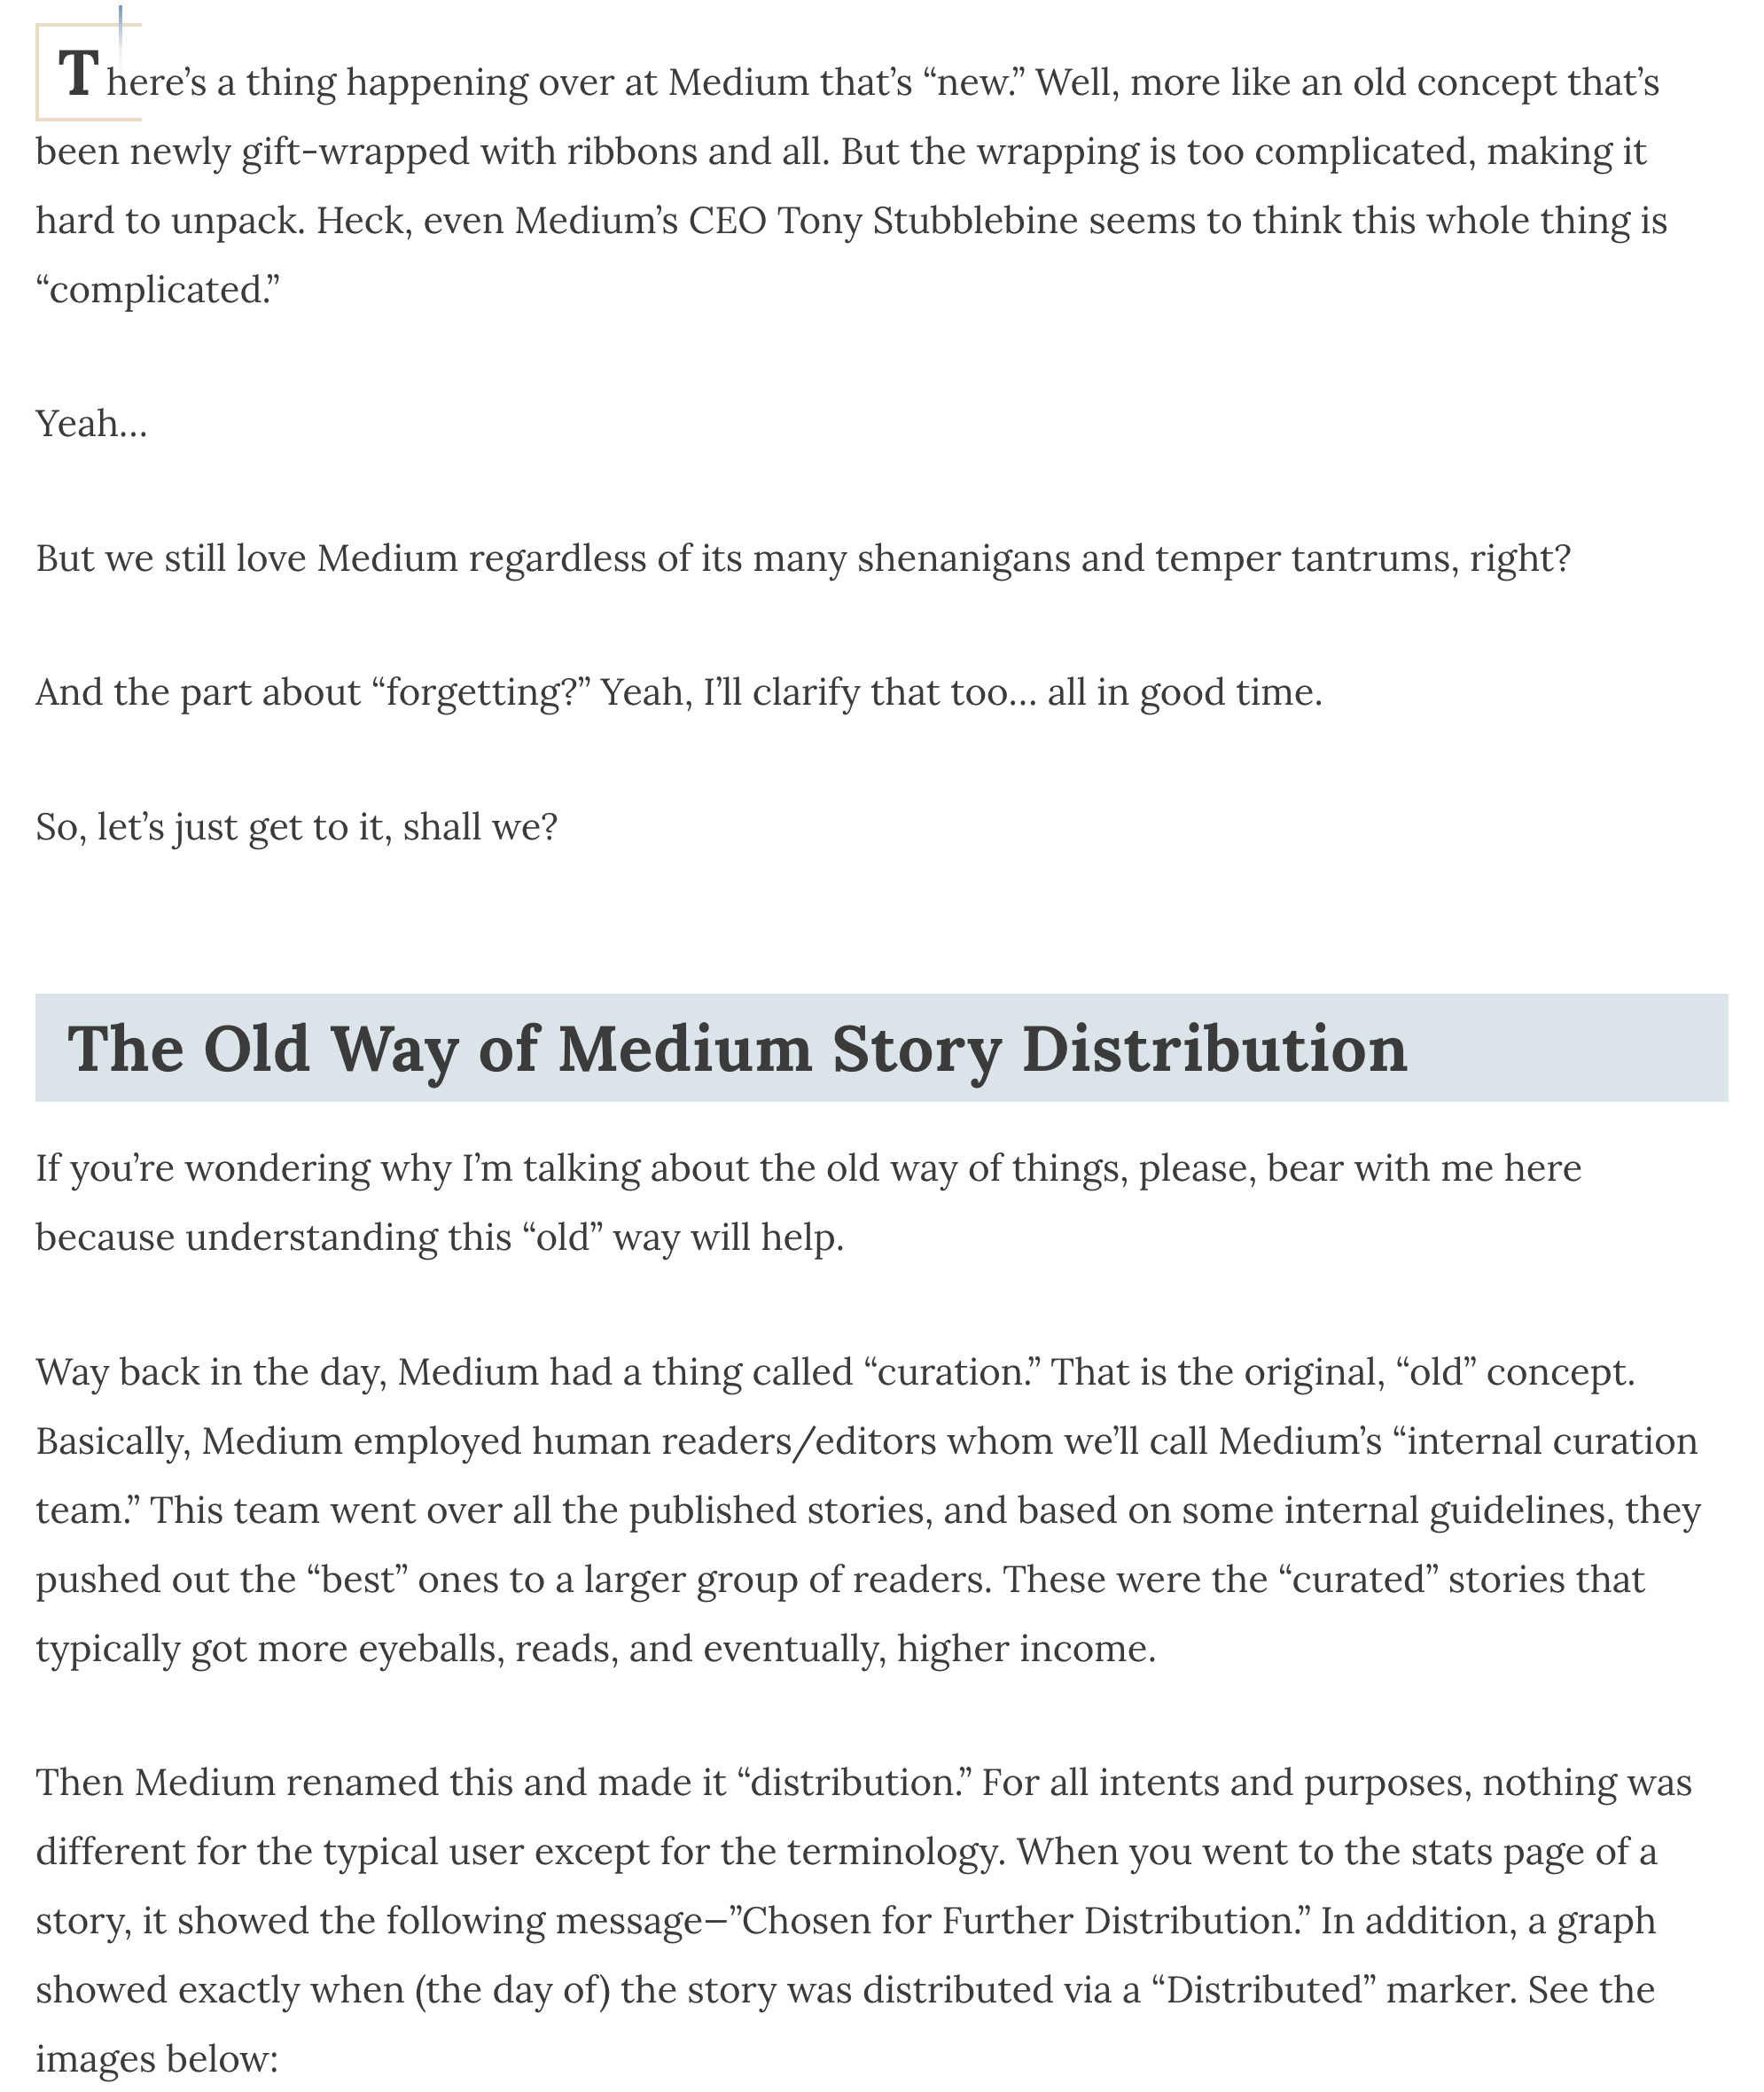
\includegraphics[width=\textwidth]{thesideblogger-p2}
\end{center}
\WillContinue
\pagebreak

\Continuing
\begin{center}
    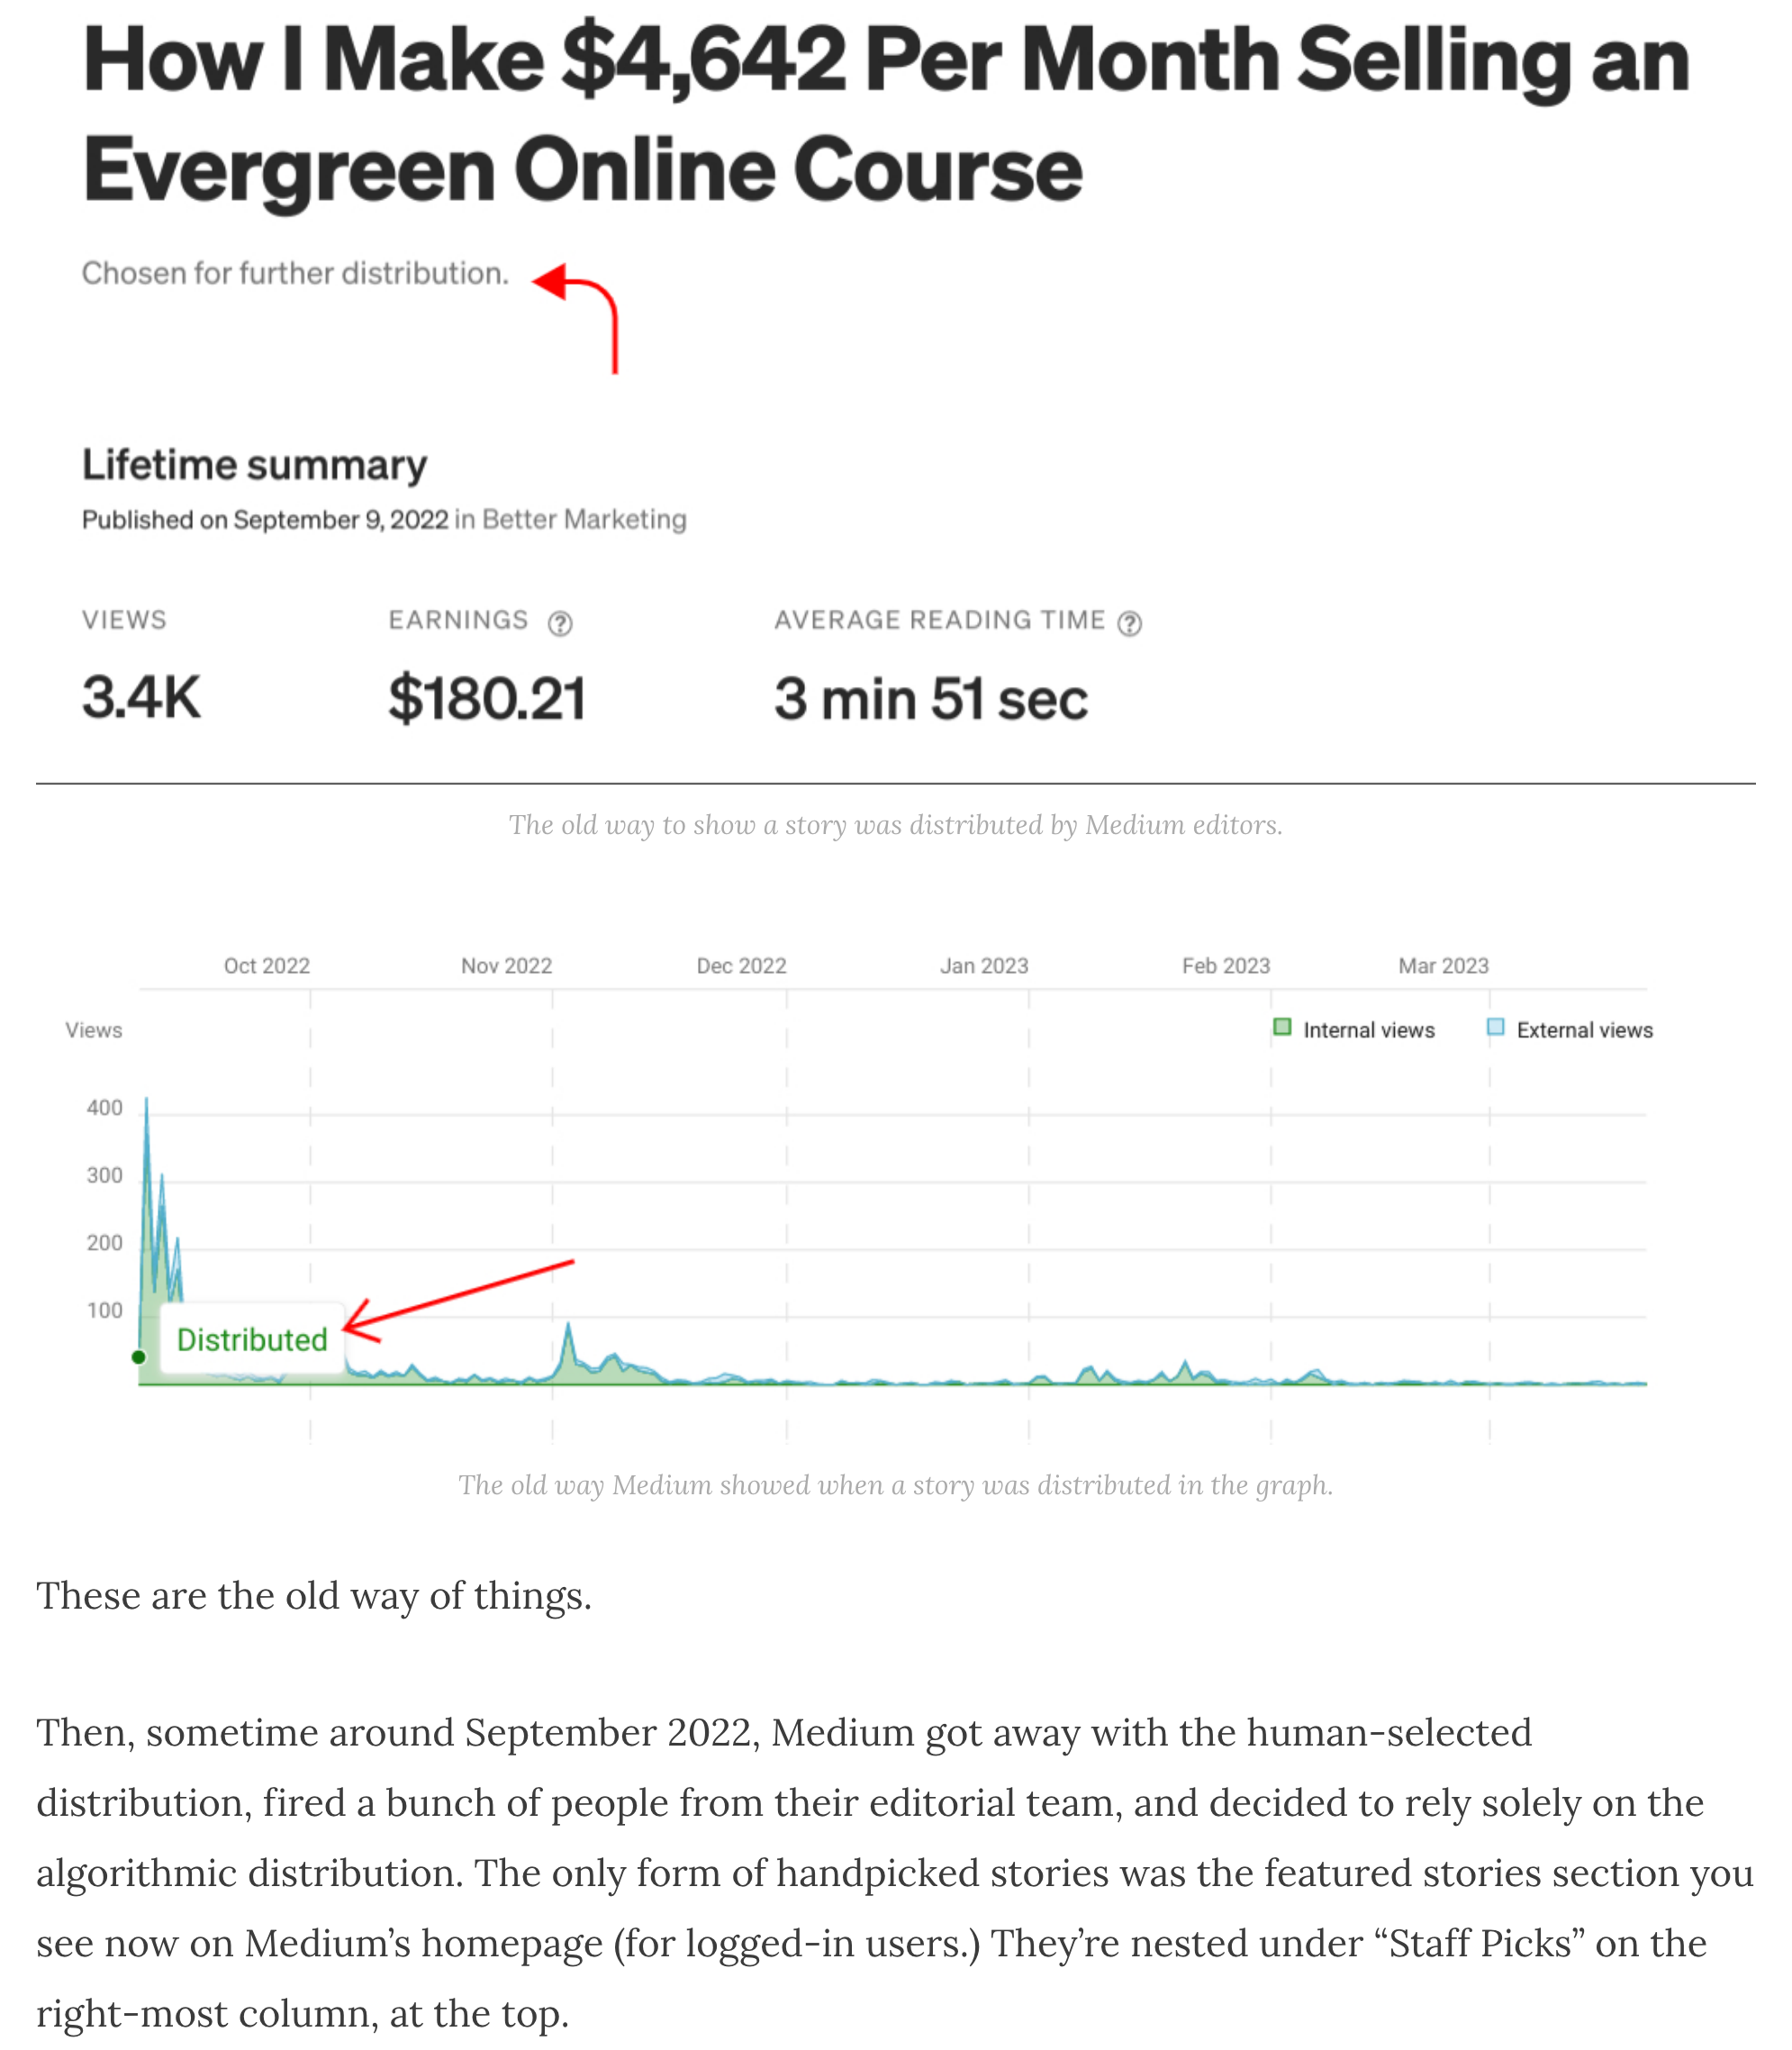
\includegraphics[width=\textwidth]{thesideblogger-p3}
\end{center}
\pagebreak


In September 2022, in the official blog on Medium,
they announced they remove one of the two signs:

\ParagraphQuote{%
    \dots This also means that stories do not need to be curated to be distributed\dots

    We've decided to stop including the `chosen for further distribution' notification
    on the story stats page going forward.%
}

This is because they employed an algorithm and reduced human curation.
This leaves the \Quote{Distributed} label on chart the only sign of being selected for the old curation program.

\begin{center}
    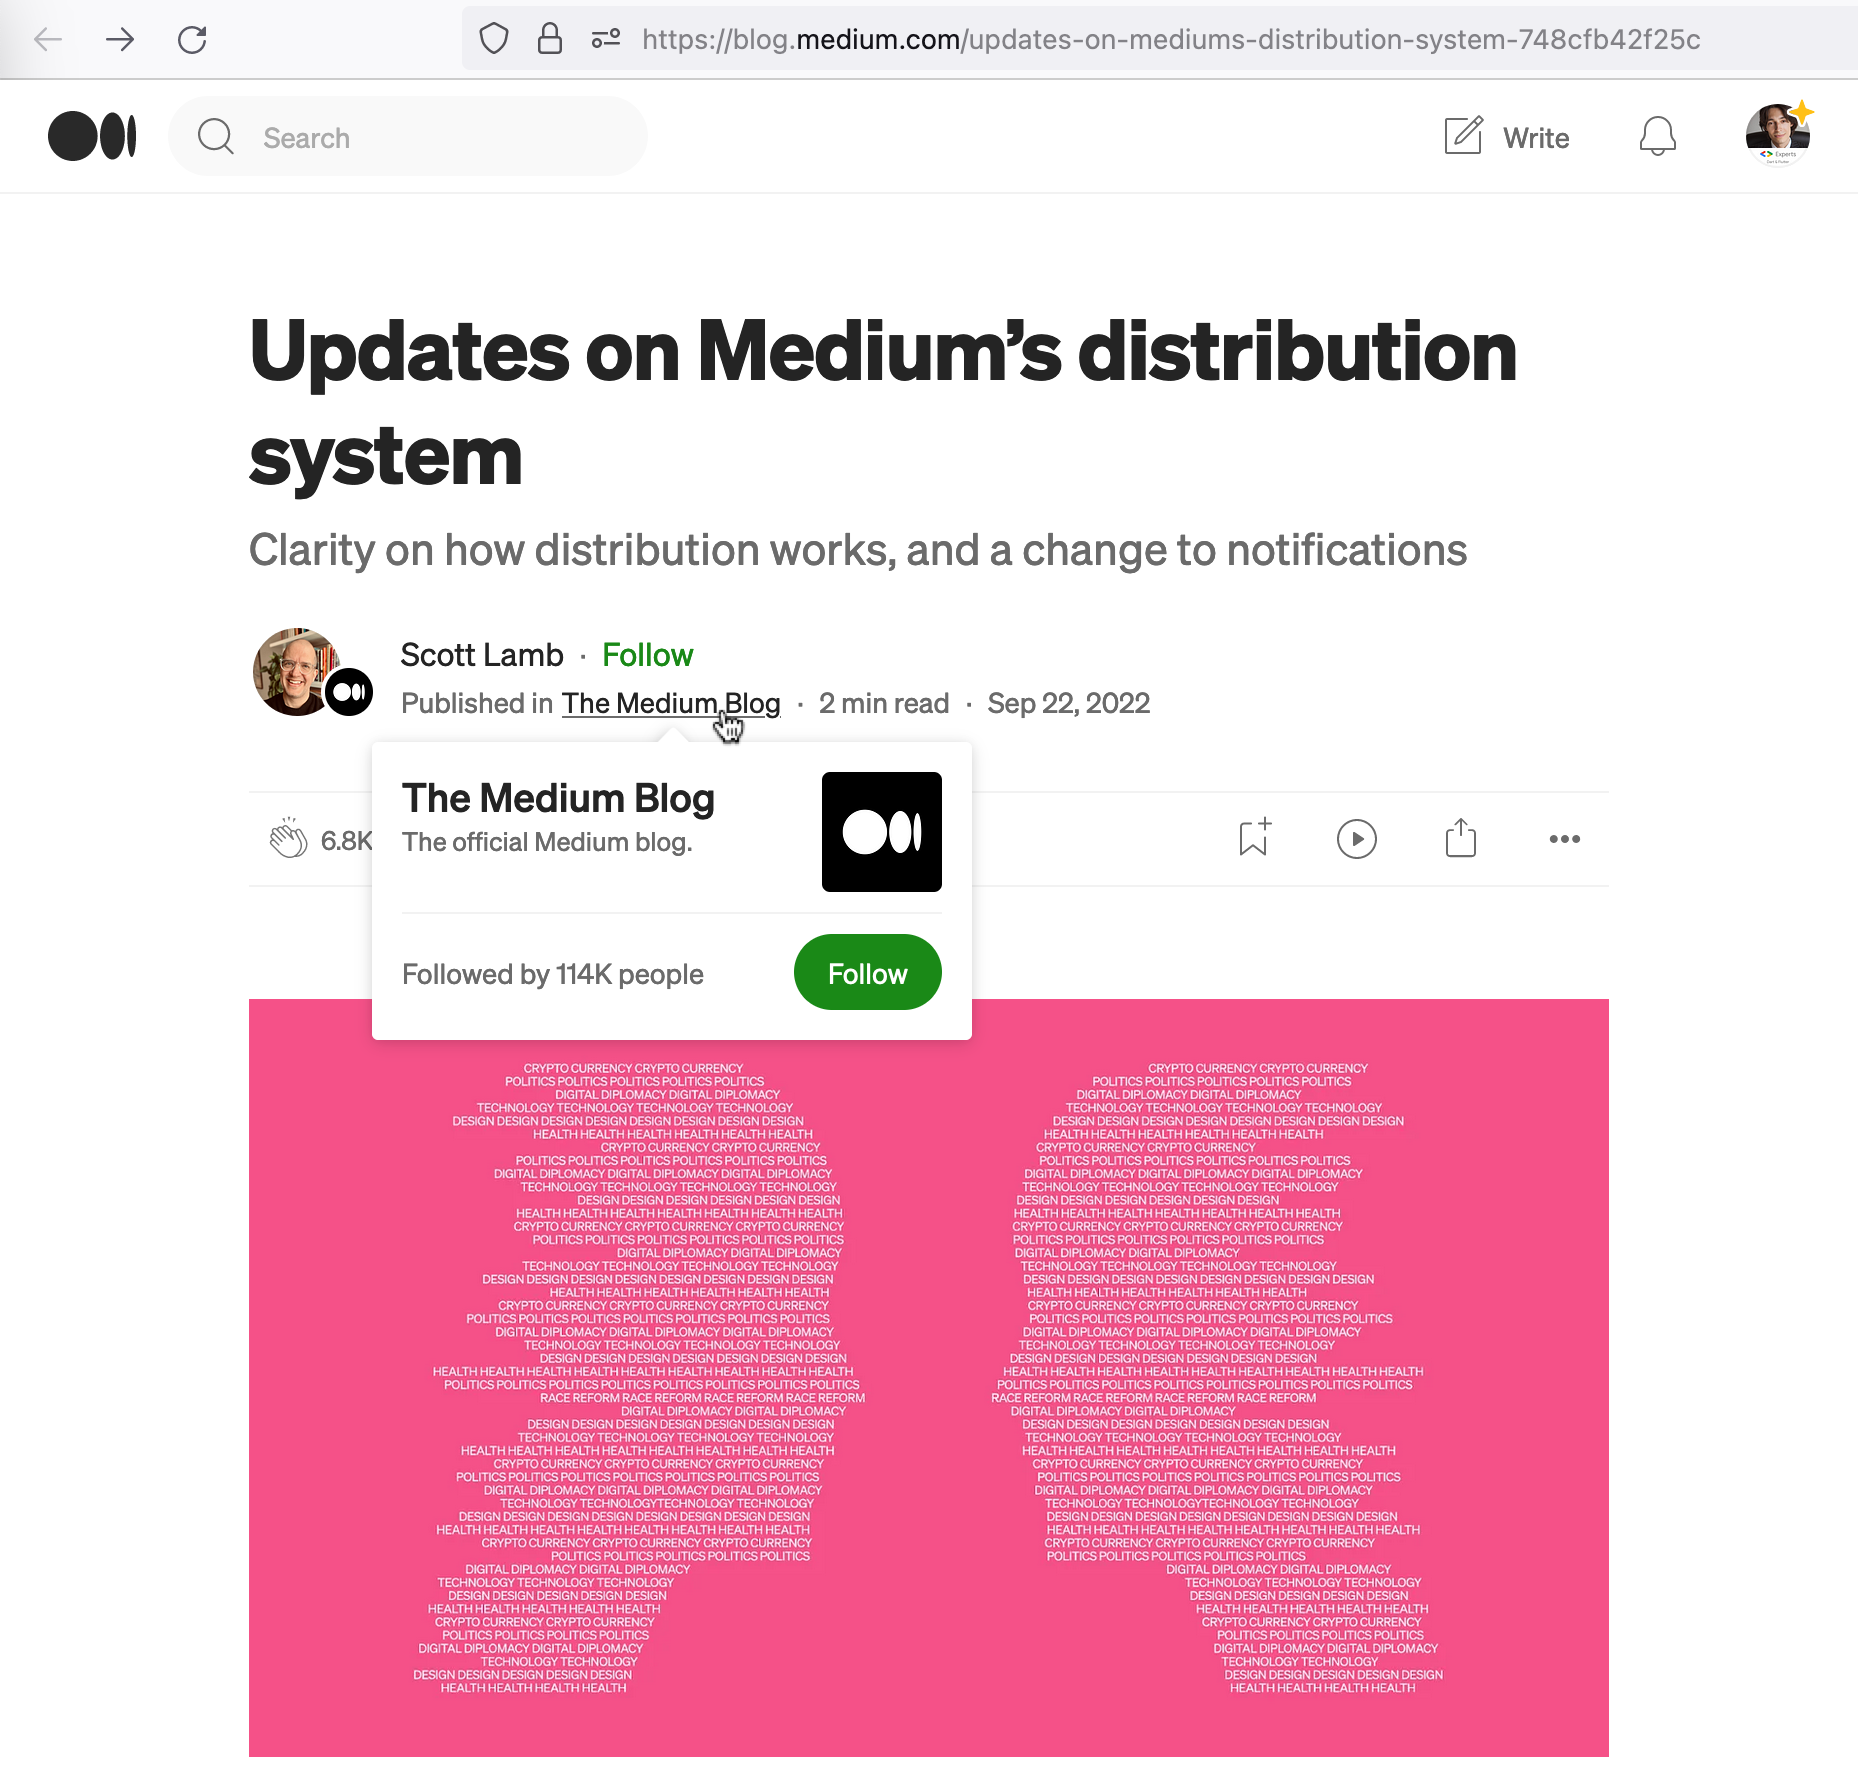
\includegraphics[width=38em]{no-more-p1}
\end{center}
\WillContinue
\pagebreak

\Continuing
\begin{center}
    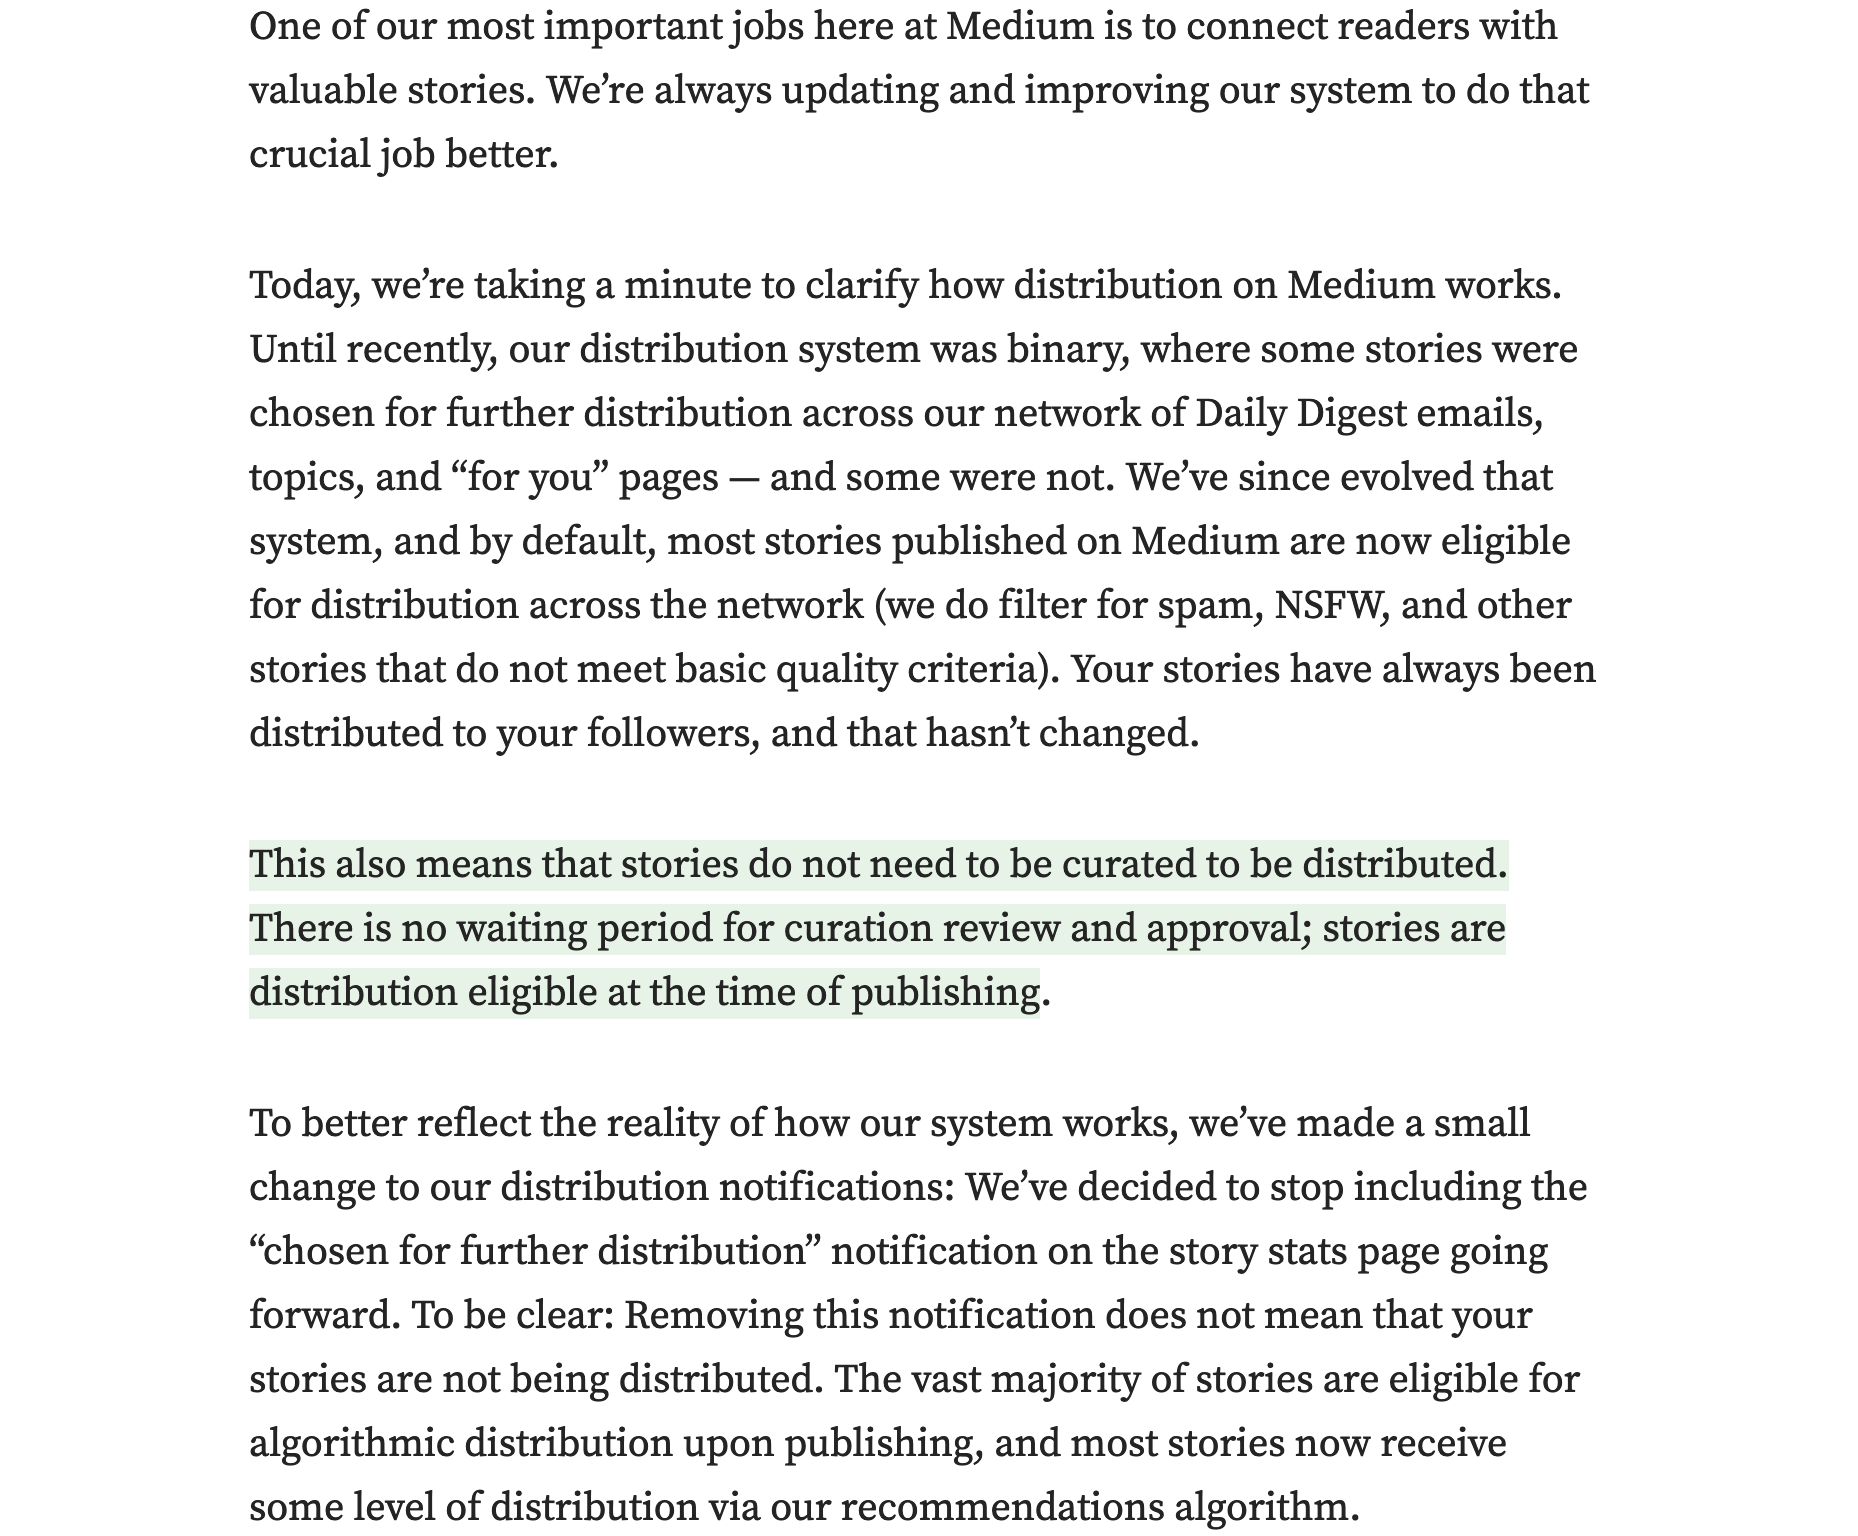
\includegraphics[width=\textwidth]{no-more-p2}
\end{center}

\pagebreak
